\documentclass[utf8, a4paper, 14pt, russian, oneside]{book}

% Размер шрифта
\usepackage[14pt]{extsizes}

% Кодировка
\usepackage[T2A]{fontenc}
\usepackage[utf8]{inputenc}
\usepackage[main=russian, english]{babel}

\usepackage{fontspec}
\setmainfont{Times New Roman}
\usepackage{sectsty}
\sectionfont{\large}
\subsectionfont{\large}

% Параметры страницы
\usepackage[left=3cm, right=1cm, top=2cm, bottom=2cm]{geometry}
\pagestyle{plain}
\linespread{1.1} % Межстрочный интервал

% Пакеты для работы с математикой
\usepackage{amsmath}
\usepackage{amsfonts}
\usepackage{amssymb}

% Вставка изображений
\usepackage{graphicx}

% Пакет для работы с таблицами
\usepackage{tabularx}
\usepackage{booktabs}
\usepackage{longtable}

% Для больших множеств
\usepackage{mathtools}

% Для работы с рисунками
\usepackage{caption}

% Для создания графов в 3 блоке
\usepackage[all]{xy}

% Для специальных символов
\usepackage{textcomp}

% Для гиперссылок
\usepackage{hyperref}

% Для таблиц
\usepackage{multirow}

\usepackage{upgreek}

\usepackage{array}
\newcommand{\mysec}[1]{
{\centering\section*{\hyperlink{toc}{#1}}}
\addcontentsline{toc}{section}{#1}
}

\newcommand{\mysubsec}[1]{
{\centering\subsection*{\hyperlink{toc}{#1}}}
\addcontentsline{toc}{subsection}{#1}
}

\newcommand{\Db}{
    \ensuremath{
        D_{\text{в}}
    }
}

\newcommand{\xb}{
    \ensuremath{
        x_{\text{в}}
    }
}

\newcommand{\yb}{
    \ensuremath{
        y_{\text{в}}
    }
}

\newcommand{\zb}{
    \ensuremath{
        z_{\text{в}}
    }
}

\newcommand{\yx}{
    \ensuremath{
        y_x
    }
}

\newcommand{\zx}{
    \ensuremath{
        z_x
    }
}

\newcommand{\cov}{
    \ensuremath{
        \mathit{cov}_{\text{в}}
    }
}

\renewcommand{\r}{
    \ensuremath{
        \mathit{r}_{\text{в}}
    }
}

\newcommand{\rang}{
    \ensuremath{
        \mathit{rang}
    }
}

\newcommand{\rhob}{
    \ensuremath{
        \rho_{\text{в}}
    }
}

\newcommand{\der}[2]{
    \ensuremath{
        \frac{\partial #1}{\partial #2}
    }
}

% Команды для настройки содержания
\renewcommand\contentsname{\center{Содержание}} % Вместо оглавления пишется содержание
\addto{\captionsenglish}{\renewcommand{\bibname}{References}}
\begin{document}

\thispagestyle{empty}
~\vspace{-2cm}\setlength{\parindent}{0cm}
\begin{center}
	
\includegraphics[scale=1.5]{../include/logo.png}\\[2pt]
	МИНОБРНАУКИ РОССИИ\\
	Федеральное государственное бюджетное образовательное учреждение\\
	высшего профессионального образования\\[5pt]
	\textbf{<<МИРЭА – Российский технологический университет>>}\\[5pt]
	\textbf{\large РТУ МИРЭА}\\[20pt]
	\hrule{}\mbox{}\\[1pt]
	\hrule{}\mbox{}\\[20pt]	
	Институт кибернетики \\ Кафедра <<Информационная безопасность>> (БК №252)\\[35pt]
	\textbf{Долгосрочное задание} \\
	по дисциплине: Математическая статистика
\end{center}
	\vspace{4in}
	Студент группы ККСО-01-19:  \qquad \qquad \qquad  \qquad     Колесников А.В.
\vspace{0.6in}
\begin{center}
Москва --- 2021
\end{center}
\newpage

\tableofcontents
\newpage

\mysec{Описание данных}

В качестве данных возьмем данные о цене на курс криптовалюты <<Ethereum>> (в долларах) в период времени с 8 ноября по 7 декабря. Объём выборки равен 30.
Пусть X - цена криптовалюты.
\begin{table}[h!]
    \centering
    \begin{tabular}{|c|c|c|}
        \hline
        № & Дата & Цена \\ \hline
        1 & 11.08 & 4619,65 \\ \hline
        2 & 11.09 & 4810,07 \\ \hline
        3 & 11.10 & 4733,36 \\ \hline
        4 & 11.11 & 4635,45 \\ \hline
        5 & 11.12 & 4724,31 \\ \hline
        6 & 11.13 & 4666,72 \\ \hline
        7 & 11.14 & 4648,63 \\ \hline
        8 & 11.15 & 4627,09 \\ \hline
        9 & 11.16 & 4570,48 \\ \hline
        10 & 11.17 & 4213,91 \\ \hline
        11 & 11.18 & 4287,80 \\ \hline
        12 & 11.19 & 3995,73 \\ \hline
        13 & 11.20 & 4298,35 \\ \hline
        14 & 11.21 & 4412,20 \\ \hline
        15 & 11.22 & 4266,51 \\ \hline
        16 & 11.23 & 4089,68 \\ \hline
        17 & 11.24 & 4340,04 \\ \hline
        18 & 11.25 & 4271,39 \\ \hline
        19 & 11.26 & 4522,21 \\ \hline
        20 & 11.27 & 4043,00 \\ \hline
        21 & 11.28 & 4101,65 \\ \hline
        22 & 11.29 & 4296,95 \\ \hline
        23 & 11.30 & 4447,77 \\ \hline
        24 & 12.01 & 4623.68 \\ \hline
        25 & 12.02 & 4586,33 \\ \hline
        26 & 12.03 & 4514,36 \\ \hline
        27 & 12.04 & 4227,76 \\ \hline
        28 & 12.05 & 4119,63 \\ \hline
        29 & 12.06 & 4199,00 \\ \hline
        30 & 12.07 & 4369,08 \\ \hline
    \end{tabular}
\end{table}
\newpage

\mysec{График динамики ряда}
Временной ряд - это собранный в разные моменты времени статистический материал о значении каких-либо параметров.

\begin{figure}[h!]
    \centering
    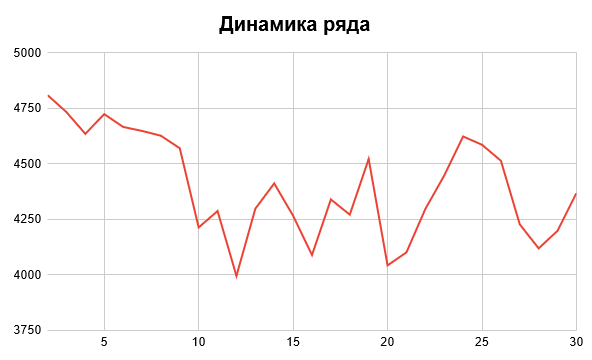
\includegraphics{img/dynamic_range.png}
    \caption{Динамика ряда.}
\end{figure}

\mysec{Автокорреляционная функция}
Автокорреляция - это обычный коэффициент корреляции для значений одной величины в разные моменты времени (лаги).
Серию коэффициентов автокорреляции уровней ряда с последовательным увеличением величины лага принято называть автокорреляционной функцией.
Автокорреляция в момент вермени $k$ вычисляется по следующей формуле:
\begin{gather*}
    r(k) = \frac{\cov(X, Y)}{\sqrt{\Db(X)}\sqrt{\Db(Y)}}
    = \frac{
        \overline{x_k \cdot x_{k-1}} - \overline{x_k} \cdot \overline{x_{k-1}}
    }{
        \sigma_k \cdot \sigma_{k-1}
    }
\end{gather*}

Если $X = \{ x_1, \ldots, x_{30} \}$, то $X_k = \{ x_1, \ldots, x_{n-k} \}, X_{k-1} = \{ x_{1+k}, \ldots, x_n \}, k \in \overline{1, \tfrac{n}{2}}, m = n - k$.

Найдём $r(1)$. Для этого необходимо вычислить вспомогательные значения:
\begin{gather*}
    X_1 = \{x_1, \ldots, x_{29}\} \qquad X_2 = \{x_2, \ldots, x_{30}\} \\
    \overline{x_k} = \frac{1}{29} \sum_{i=1}^{29} x_i = \frac{4619,65 + \ldots + 4199,00}{29} = 4410,13 \\ 
    \overline{x_{k-1}} = \sum_{i=2}^{30} x_i = \frac{4810,07 + \ldots + 4369,08}{29} = 4401,49 \\
    D_k = \frac{1}{29} \sum_{i=1}^{29} x_i^2 - (\overline{x_k})^2 = \frac{4619,65^2 + \ldots + 4199,00^2}{29} - 4410,13^2 = 53255,96 \\
    D_{k-1} = \frac{1}{29} \sum_{i=2}^{30} x_i^2 - (\overline{x_{k-1}})^2 = \frac{4810,07^2 + \ldots + 4369,08^2}{29} - 4401,49^2 = 51722,63 \\
    \sigma_k = \sqrt{D_k} = 230,77 \\
    \sigma_{k-1} = \sqrt{D_{k-1}} = 227,43 \\
    \overline{x_k \cdot x_{k-1}} = \frac{4619,65 \cdot 4810,07 + \ldots + 4199,00 \cdot 4369,08}{49} = 19445863,97 \\
    r(1) = \frac{19445863,97 - 4410,13 \cdot 4401,49}{230,77 \cdot 227,43} = 0,6617
\end{gather*}
Аналогично найдем $r(2), \ldots, r(15)$. Приведём итоговый результат в виде таблицы, опустив промежуточные вычисления:
\begin{table}[h!]
    \centering    
    \begin{tabular}{|c|c|}
        \hline
        $k$ & $r(k)$ \\ \hline
        1 & 0,6617 \\ \hline
        2 & 0,4424 \\ \hline
        3 & 0,1949 \\ \hline
        4 & 0,1888 \\ \hline
        5 & 0,1939 \\ \hline
        6 & 0,1814 \\ \hline
        7 & -0,0254 \\ \hline
        8 & -0,0599 \\ \hline
        9 & -0,2435 \\ \hline
        10 & -0,2142 \\ \hline
        11 & -0,1569 \\ \hline
        12 & -0,2445 \\ \hline
        13 & -0,4004 \\ \hline
        14 & -0,4425 \\ \hline
        15 & -0,1600 \\ \hline
    \end{tabular}
\end{table}

\begin{figure}[h!]
    \centering
    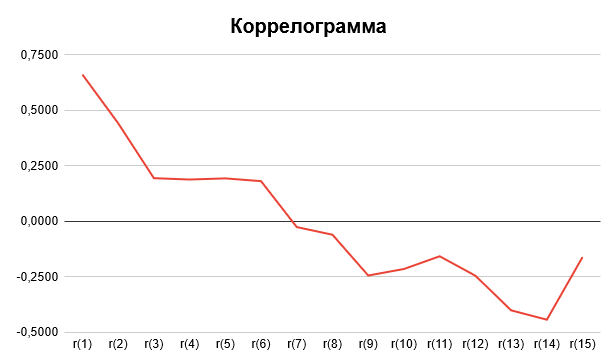
\includegraphics{img/correlogramma.png}
    \caption{Коррелограмма}
\end{figure}
Поскольку коррелограмма АКФ имеет максимум при $k=1 (r(1) = 0,6617)$, то ряд содержит только тенденцию (тренд).
Тренд - это долговременная тенденция изменения исследуемого временного ряда.

\newpage

\mysec{Уравнение тренда}
На основе коррелограммы опишем тренд линейной функцией:
\begin{gather*}
    x(t) = kt + b
\end{gather*}
Для вычисления коэффициентов $k$ и $b$ воспользуемся функцией $\varPhi(k, b) = \sum\limits_{i=1}^n (x_i - kt_i -b)^2$. Для нахождения коэффициентов $k$ и $b$ решим следующую систему уравнений:
\begin{gather*}
    \begin{dcases}
        \der{\varPhi}{k} = 0, \\
        \der{\varPhi}{b} = 0
    \end{dcases}
    \Rightarrow
    \begin{dcases}
        \der{\varPhi}{k} = -2 \sum\limits_{i=1}^n (x_it_i - t_i^2k - t_ib) = 0, \\
        \der{\varPhi}{b} = -2 \sum\limits_{i=1}^n (x_i - kt_i - b) = 0
    \end{dcases}
    \Rightarrow \\
    \begin{dcases}
        k \sum\limits_{i=1}^n t_i^2 + b \sum\limits_{i=1}^n t_i = \sum\limits_{i=1}^n x_it_i, \\
        k \sum\limits_{i=1}^n t_i + nb = \sum\limits_{i=1}^n x_i
    \end{dcases}
    \Rightarrow \\
    \begin{dcases}
        9455k + 465b = 2019386,97, \\
        465k + 30 b = 132262,79 \\
    \end{dcases}
    \Rightarrow \\
    \begin{dcases}
        k\left(9455 - \frac{465^2}{30}\right) = 2019386,97 - \frac{465 \cdot 132262,79}{30}, \\
        b = \frac{132262,79 - 465k}{30}
    \end{dcases}
    \Rightarrow
    \begin{dcases}
        k = -13,65, \\
        b = 4620,39
    \end{dcases}
\end{gather*}
Следовательно, уравнение тренда будет выглядеть следующим образом:
\begin{gather*}
    x(t) = -13,65t + 4620,39
\end{gather*}
\newpage

\mysec{Ошибки тренда}
Определим ошибки тренда $\xi_i$ по следующей формуле:
\begin{gather*}
    x_i = -13,65 t_i + 4620,39 + \xi_i \Rightarrow \xi_i = x_i + 13,65 t_i - 4620,39 \\
    \xi_1 = 4619,65 + 13,65 \cdot 1 - 4620,39 = 12,9144 \\
    \ldots \\
    \xi_{30} = 4369,08 + 13,65 \cdot 30 - 4620,39 = 158,2963
\end{gather*}

Получим следующую таблицу ошибок:
\begin{table}[h!]
    \centering
    \begin{tabular}{|c|c|c|c|}
        \hline
        $i$ & $\xi_i$ & $i$ & $\xi_i$ \\ \hline
        1 & 12,9144    & 16 & -312,2529 \\ \hline
        2 & 216,9879   & 17 &  -48,2394 \\ \hline
        3 & 153,9314   & 18 & -103,2359 \\ \hline
        4 & 69,6749    & 19 &  161,2376 \\ \hline
        5 & 172,1884   & 20 & -304,3188 \\ \hline
        6 & 128,2519   & 21 & -232,0153 \\ \hline
        7 & 123,8155   & 22 &  -23,0618 \\ \hline
        8 & 115,9290   & 23 &  141,4117 \\ \hline
        9 & 72,9725    & 24 &  330,9752 \\ \hline
        10 & -269,9440 & 25 &  307,2787 \\ \hline
        11 & -182,4005 & 26 &  248,9622 \\ \hline
        12 & -460,8170 & 27 &  -23,9842 \\ \hline
        13 & -144,5435 & 28 & -118,4607 \\ \hline
        14 & -17,0399  & 29 &  -25,4372 \\ \hline
        15 & -149,0764 & 30 &  158,2963 \\ \hline
    \end{tabular} 
\end{table}

\newpage
По этой таблице построим следующую диаграмму ошибок:

\begin{figure}[h!]
    \centering
    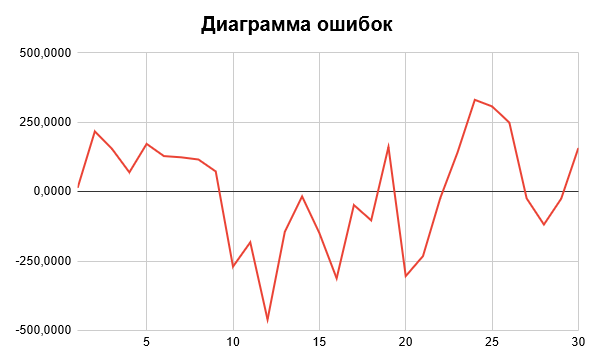
\includegraphics{img/errors.png}
    \caption{Диаграмма ошибок.}
\end{figure}

Определим коэффициент детерминации для ошибок $\xi$:
\begin{gather*}
    R^2 = 1 - \frac{\dfrac{1}{n}\sum\limits_{i=1}^n \xi_i^2}{\Db(X)} \\
    \overline{\xb} = \frac{1}{n} \sum\limits_{i=1}^n x_i = \frac{4619,65 + \ldots + 4369,08}{30} = 4408,76 \\
    \Db(X) = \frac{1}{30} \sum\limits_{i=1}^n x_i^2 - (\overline{\xb})^2 = 53330,38
\end{gather*}

Средняя ошибка:
\begin{gather*}
    \frac{1}{n} \sum_{i=1}^n \xi_i^2 = 37586,85
\end{gather*}

Коэффициент детерминации для ошибок $\xi$:
\begin{gather*}
    R^2 = 1 - \frac{37586,85}{53330,38} = 0,2952
\end{gather*}

\newpage

\mysec{Коэффициент автокорреляции ошибок с лагом 1}

Коэффициент корреляции $r_{k, k-1}(1)$ находится по следующей формуле
\begin{gather*}
    r_\xi(k) = \frac{
        \overline{\xi_k \cdot \xi_{k-1}} - \overline{\xi_k} \cdot \overline{\xi_{k-1}}
    }{
        \sigma_k \cdot \sigma_{k-1}
    }
\end{gather*}
и будет находиться между группами  $\xi_k$ и $\xi_{k-1}$:
\begin{table}[h!]
    \centering
    \begin{tabular}{|c|c|}
        \hline
        $\xi_k$ & $\xi_{k-1}$ \\ \hline
        12,9144   & 216,9879  \\ \hline
        216,9879  & 153,9314  \\ \hline
        153,9314  & 69,6749   \\ \hline
        69,6749   & 172,1884  \\ \hline
        172,1884  & 128,2519  \\ \hline
        128,2519  & 123,8155  \\ \hline
        123,8155  & 115,9290  \\ \hline
        115,9290  & 72,9725   \\ \hline
        72,9725   & -269,9440 \\ \hline
        -269,9440 & -182,4005 \\ \hline
        -182,4005 & -460,8170 \\ \hline
        -460,8170 & -144,5435 \\ \hline
        -144,5435 & -17,0399  \\ \hline
        -17,0399  & -149,0764 \\ \hline
        -149,0764 & -312,2529 \\ \hline
        -312,2529 & -48,2394  \\ \hline
        -48,2394  & -103,2359 \\ \hline
        -103,2359 & 161,2376  \\ \hline
        161,2376  & -304,3188 \\ \hline
        -304,3188 & -232,0153 \\ \hline
        -232,0153 & -23,0618  \\ \hline
        -23,0618  & 141,4117  \\ \hline
        141,4117  & 330,9752  \\ \hline
        330,9752  & 307,2787  \\ \hline
        307,2787  & 248,9622  \\ \hline
        248,9622  & -23,9842  \\ \hline
        -23,9842  & -118,4607 \\ \hline
        -118,4607 & -25,4372  \\ \hline
        -25,4372  & 158,2963  \\ \hline
    \end{tabular}
\end{table}

Получим, что $r_{k, k-1}(1) = 0,5377$.

\mysec{Оценка коэффициентов уравнений остатка}

РАссмотрим $\xi_i = a_1 \xi_{i-1} + a_0 + \varepsilon_i, i \in \overline{2, 30}$. Найдем коэффициенты $a_1$ и $a_0$ уравнения:
\begin{gather*}
    \xi_i = a_1 \xi_{i-1} + a_0
\end{gather*}

Оценим при помощи метода наименьших квадратов $\varPhi(a_1, a_0) = \sum\limits_{i=1}^n (\xi_i - a_1\xi_{i-1} - a_0)^2$.
\begin{gather*}
    \begin{dcases}
        \der{\varPhi}{a_1} = -2 \sum\limits_{i=2}^n(\xi_i \xi_{i-1} - \xi_{i-1}^2 a_1 - \xi_{i-1}a_0) = 0, \\
        \der{\varphi}{a_0} = -2 \sum\limits_{i=2}^n (\xi_i - a_1\xi_{i-1} - a_0) = 0
    \end{dcases}
    \Rightarrow \\
    \begin{dcases}
        a_1 \sum\limits_{i=2}^n\xi_{i-1}^2 + a_0\sum\limits_{i=2}^n\xi_{i-1} = \sum\limits_{i=2}^n \xi_i \xi_{i-1}, \\
        a_1 \sum\limits_{i=2}^n \xi_{i-1} + (n-1)a_0 = \sum\limits_{i=2}^n\xi_i
    \end{dcases}
    \Rightarrow \\
    \begin{dcases}
        1127438,6227 a_1 -12,9144 a_0 = 599344,7436, \\
        -12,9144a_1 + 29a_0 = -158,2963
    \end{dcases}
    \Rightarrow
    \begin{dcases}
        a_1 = 0,5315, \\
        a_0 = -5,2218
    \end{dcases}
    \Rightarrow \\
    \xi_i = 0,5315 \xi_{i-1} -5,2218
\end{gather*}

Вычислим ошибки $\varepsilon_i$:
\begin{gather*}
    \varepsilon_i = \xi_i - 0,5315\xi_{i-1} + 5,2218 \\
    \varepsilon_2 = \xi_2 - 0,5315\xi_{1} + 5,2218 = -97,2013
\end{gather*}

\newpage
По аналогии посчитаем остальные ошибки:
\begin{table}[h!]
    \centering
    \begin{tabular}{|c|c|c|c|}
        \hline
        $i$ & $\varepsilon_i$ & $i$ & $\varepsilon_i$ \\ \hline
           &           & 16 & 22,1199   \\ \hline
        2  & -97,2013  & 17 & -281,3900 \\ \hline
        3  & 140,3892  & 18 & 11,8563   \\ \hline
        4  & 122,1183  & 19 & -183,7181 \\ \hline
        5  & -16,6281  & 20 & 328,2167  \\ \hline
        6  & 109,2393  & 21 & -175,7719 \\ \hline
        7  & 67,6610   & 22 & -214,5353 \\ \hline
        8  & 67,4165   & 23 & -93,0058  \\ \hline
        9  & 82,3631   & 24 & -29,2927  \\ \hline
        10 & 221,6800  & 25 & 172,8665  \\ \hline
        11 & -167,7693 & 26 & 180,1674  \\ \hline
        12 & 67,7634   & 27 & 266,9326  \\ \hline
        13 & -378,7647 & 28 & 44,2040   \\ \hline
        14 & -130,2643 & 29 & -99,7181  \\ \hline
        15 & 67,4217   & 30 & -104,3560 \\ \hline
    \end{tabular}
\end{table}

Вычислим коэффициент детерминации для ошибок $\varepsilon$:
\begin{gather*}
    R^2 = 1 - \frac{
        \dfrac{1}{n-1} \sum\limits_{i=1}^{n-1} \varepsilon_i^2 + \xi_1^2
    }{
        \Db(X)
    } \\ 
    R^2 = 1 - \frac{
        \dfrac{1}{30 - 1} (-97,2013^2 + \ldots + -104,3560^2 + 12,9144^2)
    }{
        53330,3766
    } = 0,4935.
\end{gather*}

Для процесса $\xi_i = a_1 \xi_{i-1} + a_0 + \varepsilon_i$ условие стационарности означает, что $|a_1| < 1$, поскольку из $1 - a_1z = 0 \Rightarrow |z| = \tfrac{1}{a_1} > 1$. Тогда
\begin{gather*}
    z = \frac{1}{0,5315} = 1,88 > 1 \Rightarrow\  \text{процесс } \xi_1, \ldots, \xi_{30} \  \text{стационарен.}
\end{gather*}

\mysec{Построение авторегрессионного процесса 2-го порядка. Коэффициент детерминации}

Авторегрессионный процесс 2-го порядка:
\begin{gather*}
    Y_i = a_0 + a_1 Y_{i-1} + a_2 Y_{i-2} + \varepsilon_i, i \in \overline{3, 30}.
\end{gather*}
Оценим при помощи метода наименьших квадратов:
\begin{gather*}
    \varPhi(a_2, a_1, a_0) = \sum\limits_{i=3}^n (Y_i - a_0 - a_1Y_{i-1} - a_2Y_{i-2})^2 \\ 
    \begin{dcases}
        \der{\varPhi}{a_2} = -2 \sum\limits_{i=3}^n (Y_i - a_2Y_{i-2} - a_1Y_{i-1} - a_0)Y_{i-3} = 0, \\
        \der{\varPhi}{a_1} = -2 \sum\limits_{i=3}^n (Y_i - a_2Y_{i-2} - a_1Y_{i-1} - a_0)Y_{i-2} = 0, \\
        \der{\varPhi}{a_0} = -2 \sum\limits_{i=3}^n (Y_i - a_2Y_{i-2} - a_1Y_{i-1} - a_0) = 0
    \end{dcases}
    \Rightarrow \\
    \begin{dcases}
        -\sum\limits_{i=3}^nY_iY_{i-2} + a_2 \sum\limits_{i=3}^nY^2_{i-2} + a_1\sum\limits_{i=3}^nY_{i-1}Y_{i-2} + a_0\sum\limits_{i=3}^nY_{i-2} = 0, \\
        -\sum\limits_{i=3}^nY_iY_{i-1} + a_2 \sum\limits_{i=3}^nY_{i-2}Y_{i-1} + a_1 \sum\limits_{i=3}^nY^2_{i-1} + a_0\sum\limits_{i=3}^nY_{i-1} = 0, \\
        -\sum\limits_{i=3}^nY_i + a_2 \sum\limits_{i=3}^nY_{i-2} + a_1 \sum\limits_{i=3}^nY_{i-1} + (n-2) \cdot  a_0 = 0
    \end{dcases}
    \Rightarrow \\
    \begin{dcases}
        a_2\sum\limits_{i=3}^n Y_{i-2}^2 + a_1 \sum\limits_{i=3}^n Y_{i-1}Y_{i-2} + a_0\sum\limits_{i=3}^n Y_{i-2} = \sum\limits_{i=3}^n Y_iY_{i-2}, \\
        a_2\sum\limits_{i=3}^nY_{i-2}Y_{i-1} + a_1 \sum\limits_{i=3}^nY^2_{i-1} + a_0\sum\limits_{i=3}^nY_{i-1} = \sum\limits_{i=3}^nY_iY_{i-1}, \\
        a_2\sum\limits_{i=3}^nY_{i-2} + a_1\sum\limits_{i=3}^nY_{i-1} + (n-2)\cdot a_0 = \sum\limits_{i=3}^nY_i
    \end{dcases}
    \Rightarrow \\
    \begin{dcases}
        540183495,3 a_2 + 541709215,4 a_1 + 122833,07 a_0 = 543259744,9, \\
        541709215,4 a_2 + 563320268,8 a_1 + 127643,14 a_0 = 563930055,3, \\
        122833,07 a_2 + 127643,14 a_1 + 28 a_0 = 122833,07
    \end{dcases}
    \Rightarrow \\
    \begin{dcases}
        a_2 = 0,0259, \\
        a_1 = -0,2394, \\
        a_0 = 5364,93
    \end{dcases}
\end{gather*}

Следовательно, получим следующее уравнение авторегрессионного процесса 2-го порядка:
\begin{gather*}
    Y_i = 5364,9308-0,2395\cdot Y_i-1 0,0259\cdot Y_{i-2}
\end{gather*}

Найдем ошибки модели по следующей формуле:
\begin{gather*}
    \varepsilon_i = Y_i - a_0 - a_1Y_{i-1} - a_2Y_{i-2} = Y_i - 5364,9308 + 0,2395\cdot Y_{i-1} + 0,0259\cdot Y_{i-2}
\end{gather*}

Вычисленные значения:
\begin{table}[h!]
    \centering
    \begin{tabular}{|c|c|c|c|}
        \hline
        $i$ & $\varepsilon_i$ & $i$ & $\varepsilon_i$ \\ \hline
           &           & 16 & -36,9637  \\ \hline
           &           & 17 & -231,4777 \\ \hline
        3  & 283,9814  & 18 & -346,5806 \\ \hline
        4  & 458,5674  & 19 & -119,1522 \\ \hline
        5  & 356,1120  & 20 & -115,3366 \\ \hline
        6  & 280,9708  & 21 & 19,2158   \\ \hline
        7  & 356,5089  & 22 & -451,0060 \\ \hline
        8  & 295,1448  & 23 & -349,4947 \\ \hline
        9  & 273,3624  & 24 & -122,6339 \\ \hline
        10 & 247,4975  & 25 & 71,2755   \\ \hline
        11 & 103,5921  & 26 & 240,1050  \\ \hline
        12 & -227,7236 & 27 & 192,9407  \\ \hline
        13 & -231,6053 & 28 & 55,1421   \\ \hline
        14 & -454,1587 & 29 & -259,4049 \\ \hline
        15 & -120,5052 & 30 & -352,9323 \\ \hline
    \end{tabular} 
\end{table}

Средняя ошибка:
\begin{gather*}
    \frac{1}{n-2}\sum_{i=3}^n\varepsilon_i^2 = \frac{1}{28} \sum_{i=3}^{30} = 72223,92058 
\end{gather*}

Коэффициент детерминации:
\begin{gather*}
    R^2_{\varepsilon} = 1 - \frac{\dfrac{1}{n-2} \sum\limits_{i=3}^n \varepsilon_i^2}{\Db(X)} = 1 - \frac{72223,9206}{53330,3766} = -0,3543
\end{gather*}

\newpage

Определим с помощью уравнения $Y_i = -0,0259\cdot Y_{i-2} - 0,2395 \cdot Y_{i-1} + 5364,9308$ теоретические значения $Y_I, i \in \overline{31,38}$.
\begin{table}[h!]
    \centering
    \begin{tabular}{|c|c|c|}
        \hline
        $k$ & $Y_i$ теоретическое & $Y_i$ реальное \\  \hline
        1  & 4209,78 & 4210,21 \\ \hline
        2  & 4243,62 & 4240,67 \\ \hline
        3  & 4239,57 & 4220,39 \\ \hline
        4  & 4239,73 & 4250,97 \\ \hline
        5  & 4239,70 & 4240,48 \\ \hline
        6  & 4239,71 & 4270,15 \\ \hline
        7  & 4239,71 & 4269,12 \\ \hline
        8  & 4239,71 & 4260,78 \\ \hline
    \end{tabular}
\end{table}

При увеличении $k$ теоретическое значение будет все сильнее отличаться от реальных данных.

\mysec{Заключение}
Временной ряд содержит тенденцию.

Т.к. значения коэффициентов детерминации $R_1^2$ и $R_2^2$ находятся на достаточном расстоянии по модулю от 1, то линейное уравнение регрессии
не может достаточно точно описать данный временной ряд. Т.е. цена криптовалюты не зависит от дня.

Средние ошибки обоих моделей достаточно велики, что говорит о более сложном устройстве данной выборки.

\end{document}